\documentclass{article}

\usepackage[OT1]{fontenc}
\usepackage{mathpazo}
\usepackage[english]{babel}

\usepackage{amsmath}
\usepackage{amsfonts}
\usepackage[utf8]{inputenc}
\usepackage{graphicx}
\usepackage{float}
\usepackage{hyperref}
\hypersetup{
    colorlinks,
    citecolor=black,
    filecolor=black,
    linkcolor=black,
    urlcolor=black
}

\title{\textbf{Artificial Intelligence}}
\author{Manuel Pagliuca}

\begin{document}

\maketitle
\tableofcontents
\section{Motivation}
Artificial neural networks are information processing systems, whose structure and
operation principles are inspired by the nervous system and the brain of animals and
humans.

Artificial neural networks are studied for various reasons.

\begin{itemize}
    \item Extracting knowledge from data (\textit{phenomena, events, processes, operating environment,...}).
    \item Understanding the phenomena that I’m observing, extracting the knowledge about that phenomena.
    \item Automated construction of computational paradigms for problem solving.
\end{itemize}

The ultimate goal is to be able to have a model which allow to describe the phenomenon
that I’m observing and using this model I would like to solve the specific application problem.

There is an huge variety of application, this is the reason which AI now is so popular, and we
have so many interested and expertise in this field.

The next evolution of the economy is based on availability of solution which are extracted
from the data by analyzing the data reasoning, the only problems is that our capability
of reasoning is limited by the fact that our brain is not able to analyze huge quantity
of data, with automated system we can exploit this and make more comprehensive models that describe
the process of systems we are observing and develop more accurate solutions.

Basically, artificial intelligence is mimicking the nature. We want to take the data
analyze the data make a model, and for doing this we use techniques, we want to enrich
the analysis we are doing through sensors from environments, we can use other
specific sets of techniques.

We have the need of putting together some ideas and observation, we can define rules for reasoning, we extract the knowledge,
but we can also build knowledge through reasoning. Basically, what we want to do is to try to replicate
how the living beings observe and operate in the environment, how express, interacts.

Not only but we want to observe how the individual evolves, population evolves, in order to understand the trend
of the environment. In this broad variety of approaches is to define some techniques which mainly are
in two big categories, from the point of view of intelligence :

\begin{itemize}
    \item \textbf{Symbolic approach}
    \item \textbf{Sub-symbolic approach}, which are sub-symbolic techniques for analyze the environment
          and the systems.
\end{itemize}

During this course we are focusing on sub-symbolic reasoning techniques:
\begin{itemize}
    \item \textbf{Neural networks}, which is a simulation of a living brain.
    \item \textbf{Fuzzy systems}, which embed the definition of quantities, which are fuzzy (not defined
          in a very crisp way).
    \item \textbf{Evolutionary computing}, which is a set of techniques which mimics the natural evolution of the
          species so we can try to optimize the solution by using the basic concept of the natural evolution of the species.
\end{itemize}


\section{Neural networks}
\subsection{Biological background}
Basically, the aim of the artificial neural networks in \textit{mimicking} the behavior of our brain starts
from the fields of neural biology and neural physiology. What this discipline tries to do is to analyze the
behavior of the biological neurons cells and understand how they behave for retrieving
the information from the outer world.

The neurons use sensors and special cells to connect to the external world and get information.
As humans or other biological species, we have five senses, taking for example the eyes, they are receptors
which are able to see what a round us is, they are able to reconstruct the scene we got around us.

Basically, with artificial neural networks we are trying to replicate what \textbf{biology} does for us, in neurobiology
we build a model of what is happening in the neurons, this model describes how the neurons are
interacting together to extract the knowledge, to build memory, construct reasoning, take decisions.

In computer science we want to build this model in computer just for trying to do something similar, we want to mimic the
behavior of the natural brain in order to try to replicate in an artificial environment the same operation.

We are building the \textit{model} for neurons in the computer, in this way we are able to use these
artificial models to \textit{learn} the environment and to solve practical problem (predict possible behaviors
and solve optimization problem, like we do naturally). We also have some basis in other disciplines like
physics and chemistry since we may want to use the neural networks, also for describing physical phenomena,
not only to create reasoning in our mind but we want to create models of phenomena, this can be used for various application.
We can create an abstract model, and instead of observing the real world we can observe how the model behave in some conditions.

Neural networks and in general artificial intelligence, is a discipline of computer science and
engineering, then we use some inspirations from other discipline but the core of the theoretical aspect
of the foundation which defines the artificial neural networks this is an area which is been to computer science and engineering.
\subsection{Reasons for studying the biological background}
The reasons for studying the BB (\textit{biological background}) in computer science are two:
\begin{itemize}
    \item The \textbf{first reason} for studying the neural networks is the fact that they are a very appealing model,
          since they work in \textbf{parallel} means that they have an intrinsically extremely high \textit{parallel process capability}.
          This is why computer scientist are so attracted to this topic. Our brain in many cases find the solution immediately, this
          is fascinating, this happens because we are exploiting the parallel capability of our neural networks.
    \item The \textbf{second reason} why we are studying this technology is the fact that there is really a huge amount of \textit{practical
              application} in broad variety of area : \textit{industrial manufactory, products medicine, finances, economy, social networks, data analysis, ...}
\end{itemize}

\subsection{Neurons}
\begin{figure}[H]
    \centering
    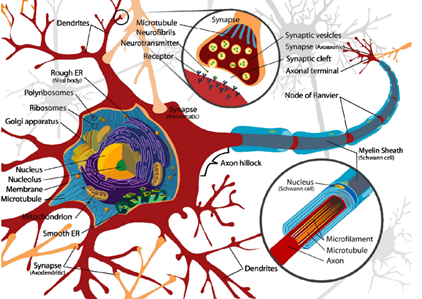
\includegraphics[width=10cm]{images/neuron1.png}
    \caption{Neuron}
    \label{fig:neurone_1}
\end{figure}

The \textit{central} part of the neuron is the part, which is managing the entire cell, this core the
nucleus is listening what is happening around the neuron,
when I have a \textbf{solicitation} from the external (other neurons or special cells related to the five senses).

When there is sufficient stimulation coming from this cells the nucleus is solicited and at a given
point the nucleus realizes that the solicitation is so high that he has to
take an \textbf{action}, the action is to send a \textit{signal} around the \textit{axon} (the long extension covered in blue),
this will lead to have a \textit{polarization} of an \textit{electric signal} which is flowing along this connection
and this will reach other neurons that are connected to the end of the axon to the synapses.

\begin{figure}[H]
    \centering
    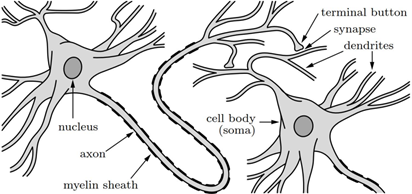
\includegraphics[width=10cm]{images/neuron2.png}
    \caption{Connection between two neurons}
    \label{fig:neurone_2}
\end{figure}

The \textbf{axon} is covered by an appropriate \textit{protein} (covered in blue) which protect the axon itself,
and make sure that the polarization that occur on the nucleus is transmitted along the axon so that this signal is able
to reach the synapse.

Basically, what we see is that the \textbf{neuron is exciting the nucleus}, which is generating the excitation along the axon,
then it will reach the terminal synapses.

Each synapse is connected to the synapses of \textit{another} neuron, so that the signals which are generated by
the nucleus and sent to the axon and then to the synapsis terminal at the terminal the synapses
are releasing some chemicals called \textbf{neurotransmitters}.

These \textit{substances} are exciting the synapses of the connected neuron, bu stimulating the synapses this excitation is
propagated from the \textbf{dendrites} to the nucleus of the other neuron, when the other cell is \textit{sufficiently excited} by
from the amount of stimulation generated by the neurotransmitter the nucleus will generate again a new stimulation
which is going along the axon and reach another neuron (and so on...).

The axon is \textit{depolarized} if there is enough excitatory input, basically this is how the signals are propagated
through the brain.

Due to the fact that each neuron can stimulate each other neurons connected to them,
this will create the \textbf{parallel processing} in our brain, so that each component will take care
of analyzing each part of the information and this is a consequence to derive a part of the total computation.

\subsection{Computer vs Human brain}
When we look to the differences between a computer and the human brain what we notice,
is that in the computer we got processors composed by many \textit{transistors}, the human brain counterpart
the got $10^11$ \textit{neurons}, the number of the latter overcomes the number of the cores in a processor.

The neurons aren’t able to process the same \textit{complex operation} of a core, but they are still so many that they
can overcome the limit of the complexity of the individual operation with the fact that they are working significantly in
parallel.

\begin{figure}[H]
    \centering
    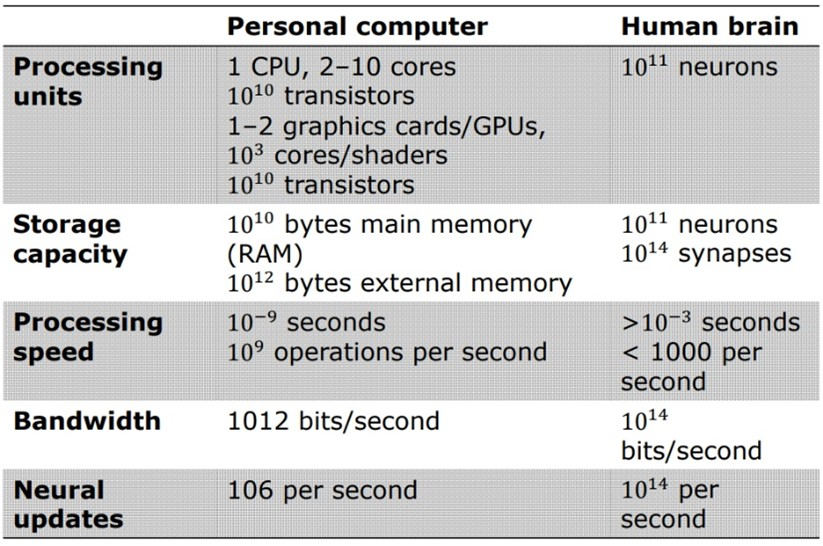
\includegraphics[width=10cm]{images/tab_pc_vs_brain.jpg}
    \caption{PC vs Human brain}
    \label{fig:tab_pc_vs_brain}
\end{figure}

The \textbf{storage} of the neurons has an immense storage potential than any other memory capacity. The \textbf{processing speed}
seems \textit{much higher} on the computer, but the parallel operation that you can do in parallel in the human brain in
the end \textit{overcome} the processing speed of the hardware of a computer.

Basically, what we can observe is that the biological neural networks are able to outperform significantly the processor that
we have nowadays, there are some researches carried out which are trying to create processors which are replicating in
hardware the operation of the biological neural networks but still the capabilities of this systems are \textit{far} from the
capability of human brain.

It may \textit{seem} in some system that they are working faster then humans, it may seem that they are running better, but actually
what you have is that you have the ability in the computer to run the algorithms and the explore the
possible (deterministic) moves in a fast way but needs some background knowledge
in order to that in a very short time.

Advantages of biological neural network:
\begin{itemize}
    \item High processing speed due to massive parallelism.

    \item Even if we have a significant amount of the biological neural network damaged, the system is
          considered \textbf{fault tolerance}, it remains functional even if larger parts of the network get \textit{damaged} (maybe some functions will be disabled).
          The other cells are able to overcome the death cells, this thanks to the elasticity of the neurons which are able
          to overcome possible damages in the structures.

    \item If more neurons are failing, the brain will \textit{degrade the performances} in a \textit{graceful way},
          it will not just stop working, will work a bit less not with the same performance and the same functionality
          but with reduced function. Only when a \textit{really massive} number of neurons is dying at that point a
          function is not working anymore.

    \item They are well suited for inductive learning (\textit{learning from examples, generalization from instances}).
\end{itemize}

What we are trying to do with artificial neural networks is to capture the parallel operation of the brain. The ability to
extract the knowledge from the data, we want to replicate these capabilities.

There are some problems due to the \textbf{ANN} (artificial neural networks), if we kill part of the architecture which
is replicating the \textbf{BNN} (biological neural networks), the ANN is \textbf{not automated to survives}, we have to
assure some physical redundance, this is a problem of the architecture we are using to execute the computation of the ANN.

What we want to do in our model is to construct a \textit{set of abstract models of the neurons} that we call
\textbf{artificial neurons}, and we like to connect them together to replicate the structure that we have in the
natural brain this is why we have the ANN, a connection of neurons that is trying to mimic the behavior of the brain.

The complexity of the brain is so high that is actually difficult to replicate everything in ANN,
what we are doing is to replicate a specific function of the brain which is able to solve a specific application
problem that we have.

\subsection{Threshold Logic Units}
This is the first \textit{abstract model} for an artificial neuron of the brain.
A \textbf{threshold logic unit} (TLU) is a \textit{processing unit} (neuron) with several inputs.
It can solve a very simple set of problems.

We have a \textbf{core} (the neuron) with several \textit{inputs} that are reaching the neuron, and we have the
\textit{output} which is delivered to the subsequential neurons which are connected with it.
A TLU is a processing unit in which the output is governed by a threshold $\theta$, if it has a \textit{sufficient excitation}
from the inputs, then the TLU became \textbf{active} (value $1$) and generates the output $y$.

\begin{figure}[H]
    \centering
    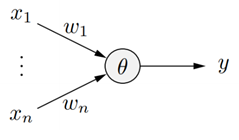
\includegraphics[width=6cm]{images/tlu.png}
    \caption{Threshold logic unit}
    \label{fig:tlu}
\end{figure}

We have $n$ inputs identified by $x_1,…,x_n$ the unit is generating only one output $y$ each input is \textbf{not}
delivered directly to the core of the TLU, but each input is \textbf{weighted}, some are more relevant,
and others are less relevant (exactly how we are doing when we consider the data from the external world).

\begin{figure}[H]
    \centering
    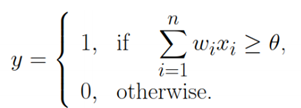
\includegraphics[width=6cm]{images/tlu_working_system.png}
    \caption{TLU conditions}
    \label{fig:tlu_conditions}
\end{figure}

This means that our problem is depending on the most important information, this is what happens in the real world.

In the ANN we are replicating the relevance of the individual input, we can control how much each input is actually
important to influence the generation of the output, to do this we use a weight $w$ for each of the input so
that the TLU will not see exactly the input but will see a weighted input, this will allow the modulation of
each input by giving to each of them the appropriate importance during the generation of the final output.

When the TLU is solicited enough it will generate an output $y$ that will be delivered to the \textit{terminal synapse}
to another neuron.
\begin{itemize}
    \item If the \textbf{excitation is enough}, mathematically means that the weighted summation is greater
          than a thresh $\theta$, we generate $1$ (the neuron is active).
    \item If the \textbf{excitation is not enough} for overcoming the threshold $\theta$, we generate $0$.
\end{itemize}

This model that tries to represent what is happening in the BNN from two scientists, also called the \textbf{McCulloch-Pitts neuron}.
\subsubsection{Conjunction example}
The result is equal to $1$ only when the two outputs are equal to $1$.
There is not a standard way to select the threshold $\theta$, we have to choose that in base of the
function that we want to implement. In this case I have to select a $\theta$ which is greater than the biggest weight.

$$x_1\land x_2$$

\begin{figure}[H]
    \centering
    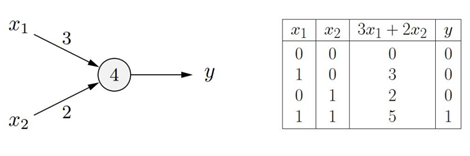
\includegraphics[width=10cm]{images/conj_TLU.png}
    \caption{Conjunction TLU}
    \label{fig:tlu_conjunction}
\end{figure}

\subsubsection{Implication example}
I can choose the value of the threshold in order to have the proper function, in this case applies on the same ways.
\textit{How can I choose the interconnection weights?}

The problem is that there are no general rules, I choose the weights according to the intrinsic relevance of each
input variable.

\textit{How can I do that when we have a high number of inputs?} we will see that there is a procedure for doing that.
$$x_2\rightarrow x_1$$
\begin{figure}[H]
    \centering
    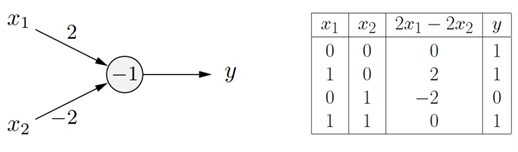
\includegraphics[width=10cm]{images/impl_TLU.png}
    \caption{Implication TLU}
    \label{fig:tlu_implication}
\end{figure}

\subsubsection{Multiple inputs example}
In this case we can see that we have three possible inputs, we can discriminate the
inputs in excitatory input and inhibitory input. The first tries to contributes
to the final computation of the neuron in such a way that the results
will be greater than the threshold, the other neuron does the opposite.

\begin{figure}[H]
    \centering
    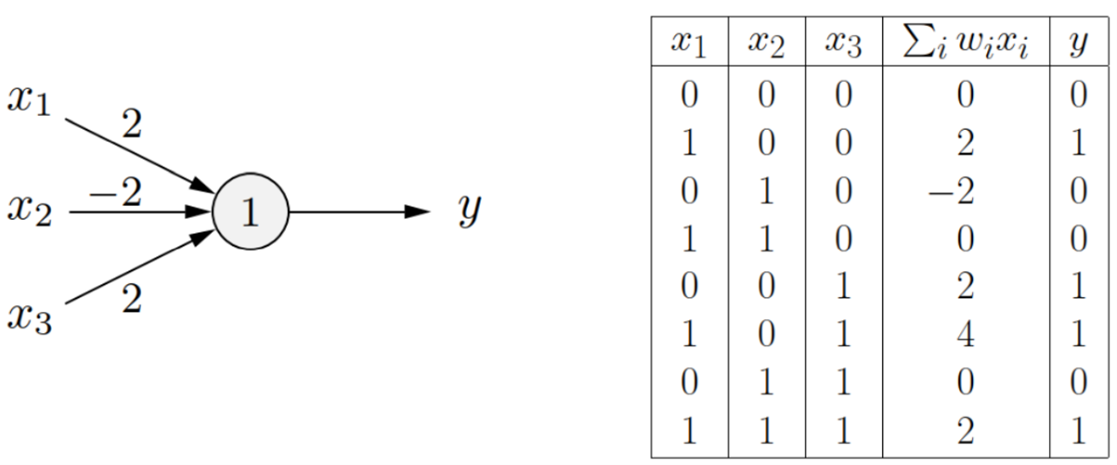
\includegraphics[width=10cm]{images/complex_TLU.png}
    \caption{Three-input TLU}
    \label{fig:tlu_3_input}
\end{figure}

\subsection{Geometric interpretation}
The geometric interpretation is significantly helpful to derive a \textit{method} to
configure the threshold and the weights starting from the data. We will consider a
single and simple TLU, we will try to understand how we can interpret the
behavior of the TLU in a geometrical way.

You know that is possible to represent a straight line on a plane in any of
the following forms :
\begin{figure}[H]
    \centering
    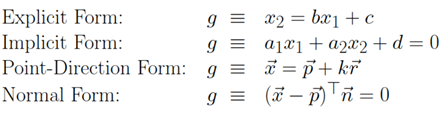
\includegraphics[width=10cm]{images/geom_interp.png}
    \caption{Different form for representing a straight line}
    \label{fig:line_repr}
\end{figure}

If i \textbf{implicit form}, where you have a weighted combination of the two variables plus a
possible threshold, a vector representation in point-direction form and normal form.
Any of this is fine to represent a straight line in the plane, we are considering just
two variables $x_1$ and $x_2$, and use one of the many representations.

\begin{figure}[H]
    \centering
    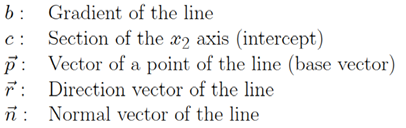
\includegraphics[width=9cm]{images/geom_interp_impl.png}
    \caption{Implicit form representation legend}
    \label{fig:line_impl_form_legend}
\end{figure}

\begin{figure}[H]
    \centering
    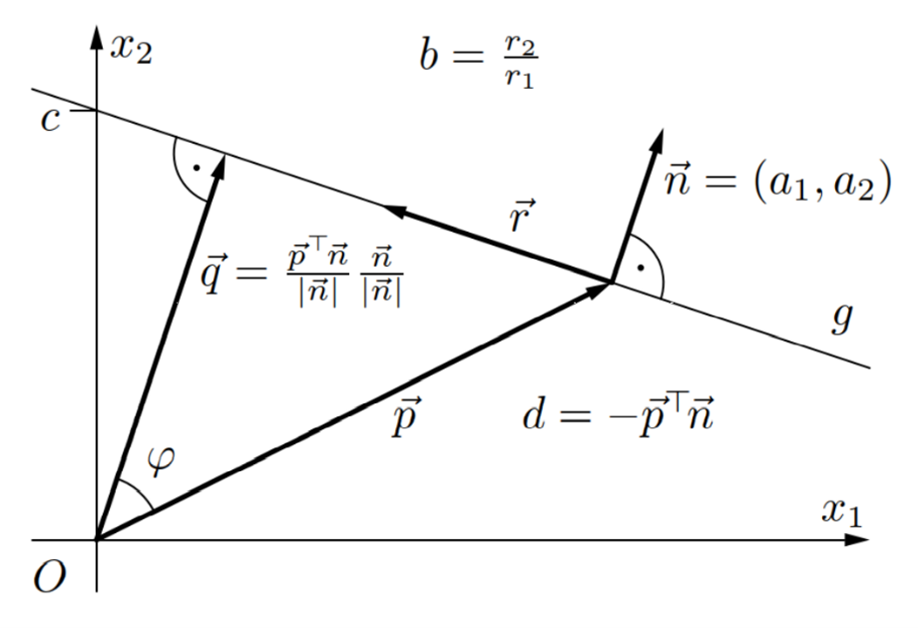
\includegraphics[scale=1]{images/geom1.png}
    \label{fig:geom_1}
\end{figure}

In the case of the \textit{explicit/implicit form} the $\vec{b}$ is the \textbf{inclination}
(or \textit{gradient}) of the straight line in respect of the horizontal axis,
and $c$ is the intercept of the vertical axis.

If we look to the normal $\vec{n}$ we want to pick the vector which is \textit{orthogonal}
to the straight line. The straight line is represented by all the points which starts from the
origin and has a quantity in the direction of the normal. The vector $\vec{p}$ identifies a
point in the example, we consider that point belonging to our straight line,
the distance of the straight line respect to the origin $O$ is given by $|\vec{q}|$ which is
the projection of $\vec{p}$ on straight line $g$.

\begin{figure}[H]
    \centering
    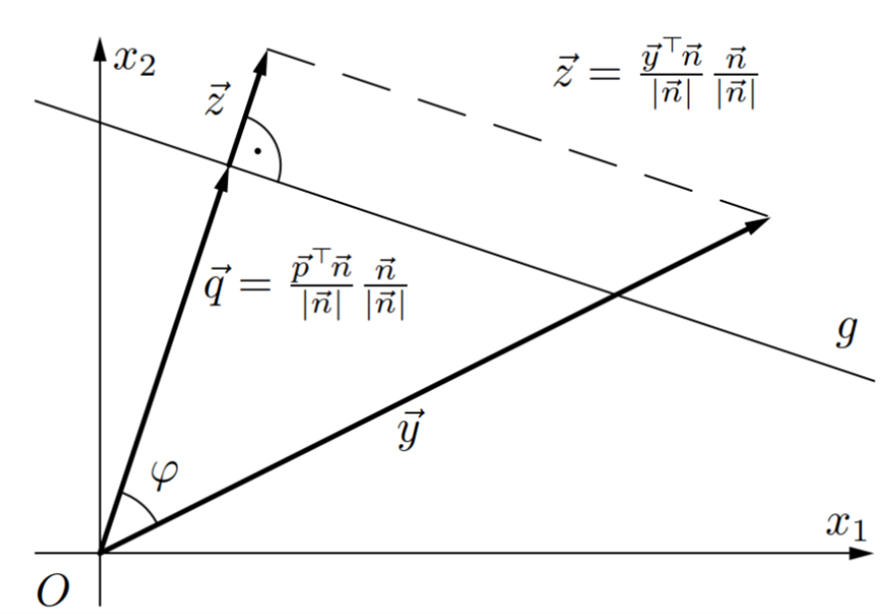
\includegraphics[scale=1]{images/geom2.png}
    \label{fig:geom_2}
\end{figure}

Considering this other graphical representation it is possible to know on which side
a points lands. If we take the vector representing $\vec{y}$ a point,
and i compute the projection in the direction of the normal, the projection
of this is the vector $\vec{z}$.

To understand on which side the points are, i just need to see if the vector $\vec{z}$ (which is the
projection of our point) is shorter or longer than the point i observe on the straight line, which
is pointed by $\vec{q}$. This means that all points (expressed by a vector) which have a \textbf{module}
higher then the projected point onto the straight line ($\vec{q}$), are part of the plane above the
straight line (they will \textit{satisfies} the solution), viceversa, they will be below the plane if the
module will be shorter then $\vec{q}$ (they won't satisfy the condition).

Basically the straight line which defines the behavior of my TLU, splits the plane in two parts (since i'm
considering only $x_1$ and $x_2$). All the points which distance is greater then

\begin{figure}[H]
    \centering
    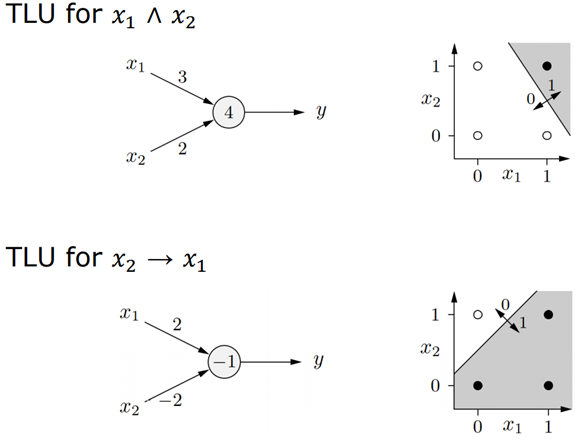
\includegraphics[scale=0.8]{images/tlu_examples_interp.png}
    \caption{Solution of the \textit{conjunction} and \textit{bi-implication}}
    \label{fig:example_interp}
\end{figure}

Now Let’s go back to the two examples that we have seen before,
starting with the conjunction, in this means that I have three points in which the output
has to be $0$, and one point where the result is $1$. This means that if I represent the straight
line with $x_1=3$, $x_2=3$ and the intercept equal to $4$ i will draw a line which is actually
separating in a clear way the element in which the output is equal to $1$ from the values
where the output is equal to $0$.
\newline
\newline
For the case of three variables, this is more complex, we need to generalize this idea moving from
a plane to a three-dimensional space. Think about the three axis and look at the combination of the
dots, you need to set a plane, so you have to separate one set of inputs for which the output has
to be equal to $1$ from the set of inputs combinations where the output is equal to $0$.

\begin{figure}[H]
    \centering
    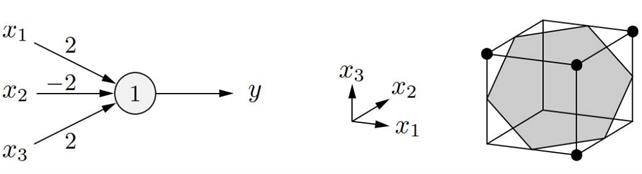
\includegraphics[scale=0.6]{images/three_input_sol_example.png}
    \caption{Solution of the complex TLU}
    \label{fig:example_three_sol}
\end{figure}

Basically, if you represent the plane using these information’s you will have this
kind of plane (that looks like a hexagon) dividing the solution from the $0$ values.

\textit{So how we choose the threshold and interconnection weights?} I have to look at geometrical
distribution of the points for the combination of the input which the output must be equal to $1$
and the one where the output must be equal to $0$, I have to take a straight line or plane and I
need to position the divisor in a way that I clearly separate the two groups. If I can do that,
that set of values (inputs and threshold) are the one that I need to use in my ANN.

\begin{figure}[H]
    \centering
    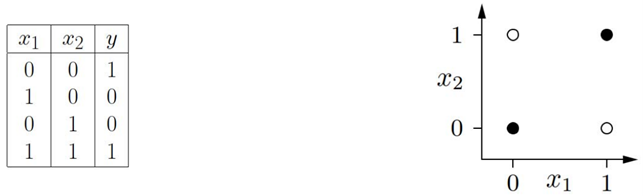
\includegraphics[scale=0.6]{images/bi_implic_no_sol.png}
    \caption{The bi-implication problem}
    \label{fig:bi-impl-problem}
\end{figure}

Let’s analyze another example, the bi-implication problem, this problem results in this kind of
distribution in the plane, as you can see it is not possible to separate these points with a
straight line. As a consequence, we don’t have any TLU for solving this problem, even if this is
a simple problem. We have to introduce some notions for understanding the reasons behind
this problem.
\subsubsection{Linear separability}
Two set of points in the \textbf{Euclidean Space}, consider $x_1, x_2,...,x_n$ as the variable for
the TLU, since we have n possible inputs you are analyzing a problem represented in $n$
dimensional Euclidean space.

If you have in this Euclidean space two set of points they are \textbf{linearly separable},
if and only if there exists at least one point, line, plane or hyperplane, such that all
points of the first set lie on one side and all points of the other set lie on the
other side of this point, line, plane or hyperplane.

The point sets can be separated by a linear decision function.

If you are in a mono dimensional space you have one input only,
your Euclidean Space is a line, you have one point on this straight line which is separating
your space the line in two parts, the output is one, for the other point the output is $0$.
If you have a plane, we have two input variables, we have to find a plane that separates
the two sets of points.
\subsubsection{Convex hull}
A set of points in the Euclidean Space is called \textbf{convex} if it is non-empty and
connected and for every pair of points in it every point on the straight-line segment
connecting the points of the pair is also in the set.

A \textbf{convex hull} of a set of points $X$ in a Euclidean Space is the smallest convex set of
points that contains $X$. Alternatively, the convex hull of a set of points $X$ is the intersection
of all convex sets that contain $X$.
\subsection{Solution of the bi-implication problem}
Two sets of points in Euclidean Space are linearly separable if and only if their convex hulls
are disjoint. In the bi-implication problem, the convex hulls are the diagonal line segments.

They share their intersection point and this means that they are not disjoint, therefore
the double implication is not linearly separable.

\begin{figure}[H]
    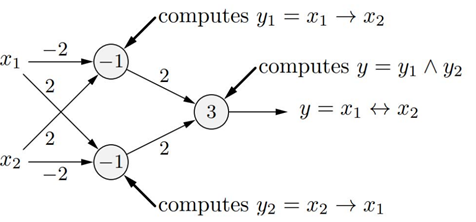
\includegraphics[scale=0.8]{images/sol_bi_implic_problem.png}
    \centering
    \caption{TLUs to the bi-implication problem}
\end{figure}
What we can do is putting together more neurons to try to address more complex problem where
one neuron can’t solve. We are creating a network of TLUs, we are splitting the problem in two
sub problems.

The problem of implication can be solved with a single TLU, we create a more complex structure
in which are able to solve the problem.

Let’s see what happens geometrically, the two points $a$ and $c$, are going to be separated
from the first two  TLUs, I set one of the TLU so that all points which are below the straight
line represented by $g_2$ fives and output equal to $1$, and then i set a second straight line
represented by $g_1$ where all points are all over the straight line the values are equal to $1$,
and then I merge this information.

\begin{figure}[H]
    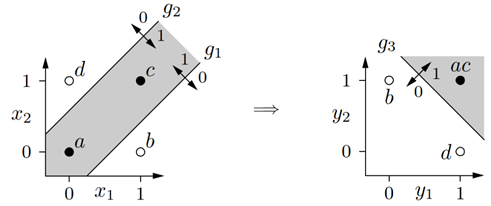
\includegraphics[scale=0.8]{images/sol_bi_implic_problem_graph.png}
    \centering
    \caption{Solution of the bi-implication problem}
\end{figure}

I combine these information from the previous group in the third neuron so that I transform
the representation of the information, I can merge the information of the points $a$ and $c$,
so that both the output of the two TLU is equal to $1$ is represented by one points (in this case
they are the same) and then I have the two other points $b$ and $d$ which are in both the parts
above and below the line, for them the solicitation is not enough to generate an output
equal to $1$, as a consequence I obtained a linear separability.

I transformed the stripe in a semi plane with the third TLU, which identifies the linear
separability, I don’t have that propriety only with the first TLU but also with the second,
both TLUs allow me to partition the first space in three parts.

\subsection{Arbitrary boolean functions}
I can work with any arbitrary \textbf{Boolean function}; in this example I have a
Boolean function of three variables. I have these values of the value $y$ according to the formula.

\begin{figure}[H]
    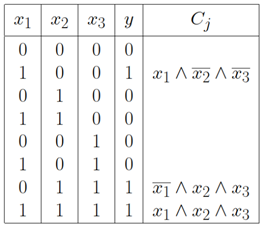
\includegraphics[scale=1.0]{images/arb_bool_funcs.png}
    \centering
    \caption{Table of values}
\end{figure}

What we can do is to build a network of TLUs that allow me to compute each of the component
for which the output has to be $1$ and then with a conjunction unit I put together all
the possible value with a or for merging the individual TLUs.

\begin{figure}[H]
    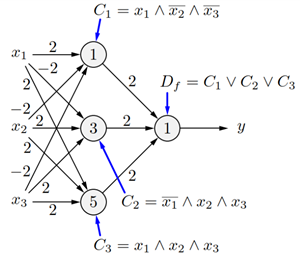
\includegraphics[scale=1]{images/arb_bool_funcs_graph.png}
    \centering
    \caption{Network of TLUs solving the boolean function}
\end{figure}


\subsection{Training TLUs}
The geometric interpretation that we have seen before about the operation of TLUs gives us the
understanding of how we can place the various parameters for our networks in order to
construct TLUs with $2$ and $3$ inputs.

But this makes sense when we are using $2$ or $3$ input, but this is something that is not
feasible when we are having more than three inputs, also this is not an automated method.

We want an automatic method for visualizing the space and points in the space, especially when
we have more then $3$ inputs.

What we want to do is to have an automatic way which adjusts the weights and the threshold
of the network so that I can reach the desired solution (if the two sets are linearly separable).

The \textbf{automatic training} of TLUs consist in the fact that we can start from a random value
of the weights and threshold, and then when we want to configure a TLU we need to evaluate
the error that we are generating at the output (of the TLU) in respect to the input pattern
that we have presented.

Basically, we have chosen randomly the threshold, the TLU generates an output, we evaluate
the error respect to the desired output, and then we try to adjust the weights and the
threshold to reduce the error.

We repeat this operation for all inputs until the error is really reduced or vanished.
\begin{enumerate}
    \item Start with random values for weights and threshold.
    \item Determine the error from the output of the TLU.
    \item Consider the error as a function of the weights and the threshold $e=e(w_1,...,w_n,\theta)$.
    \item Adapt weights and threshold so that the error becomes smaller.
    \item Iterate adaptation until the error vanishes.
\end{enumerate}

\subsubsection{Negation example}
\begin{figure}[H]
    \centering
    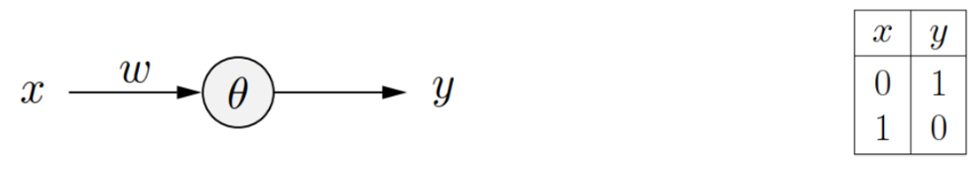
\includegraphics[scale=1]{images/neg_example.png}
    \caption{TLU that perform negation}
    \label{fig:neg_example}
\end{figure}
$$\neg x$$
In this case we have two really simple parameters, the weights and the threshold.
Let’s represent the error for all possible weights and all possible threshold at least
for a subset that we are interested in analyzing. Let’s consider the $x=0$, in this case
the desired output is $1$, if we take $w=2$ and we multiply it by $0$ the weighted input
will be $0$.

\begin{figure}[H]
    \centering
    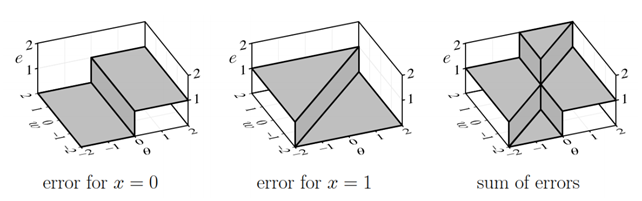
\includegraphics[scale=0.7]{images/errors_exampl.png}
    \caption{Diagrams of the errors expressed in terms of $\theta$ and $w$}
    \label{fig:neg_tlu_errors}
\end{figure}
Let's consider the first diagram on the left, with the various values of $\theta$ and $w$, and
with an input value of $x=0$.
Let's see the error that we have with the various possible combinations, we see that
for any values of the weight where the threshold is \textit{less} than zero, the \textbf{error}
is zero. Viceversa, for any value of the weight for a $\theta$ greater or equal to zero, the
error is one (a \textit{plateau}).

Now let's consider $x=1$, we are on the central diagram, in the left triangular part
of the domain there will be the error of $1$ defined $\forall w$.

Let's try to sum the errors and see what we obtains: we get an intersection for the error
equal to one, and also an intersection for the error equal to \textit{two} (which is strange,
since the error in this kind of example is always $1$ since the $y$ output is binary, but there
we are talking about a sum).

The only part where the error is equal to zero is a small triangle on the bottom. The problem
with this definition of the error is that is not suited for define an algorithm which allow
me to find the zero error.

\begin{figure}[H]
    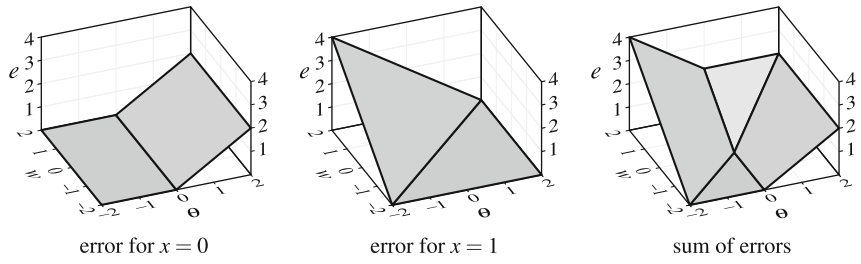
\includegraphics[scale=0.5]{images/desc_2_of_error.png}
    \centering
    \caption{Output error modified as function of weight and threshold}
\end{figure}

What i can do is modify the description of the error and consider that for each value
of the input i will not have just the error which is $1,0$ or $2$, but i will consider
a covering and continuos \textbf{surface area} (such that is possible to increase progressively
the error).

\begin{figure}[H]
    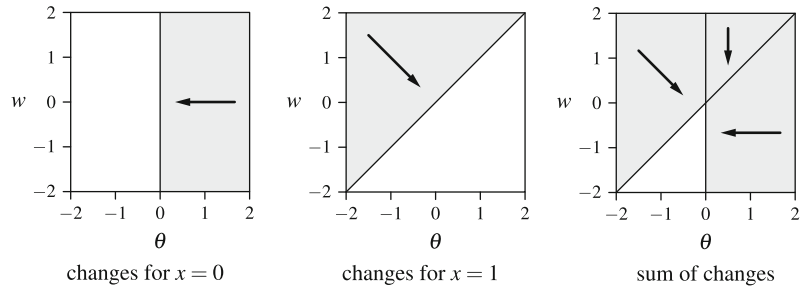
\includegraphics[scale=0.6]{images/desc_2_of_error_topview.png}
    \centering
    \caption{Top view output error modified as function of weight and threshold}
\end{figure}

So i can start from a random point and iteratively adapt parameters according to the direction
corresponding to the current point, i will stop if the error vanishes.

There are two ways of training a neural network:
\begin{itemize}
    \item \textbf{online learning}, we receive the learning pattern at time from the
          external environment, we compute the parameter corrections for this learning pattern (like
          we saw in the negation example) and in the end we apply the parameter corrections. In
          case of the \textit{negation}, first we adapt the weight and the threshold according to the left diagram,
          then we adapt them according to the middle diagram, then we adapt them again
          according to the left diagram and so forth until the error vanishes.

    \item \textbf{batch learning}, consists in not applying the changes immediately after every
          training example, but aggregating them over all training examples. Only at the end of
          a (learning/training) epoch, that is, after all training examples have been traversed,
          the aggregated changes are applied. Then the training examples are traversed again
          and at the end the weight and the threshold are adapted and so forth until the error
          vanishes.
\end{itemize}

\subsubsection{Delta rule (Widrow-Hoff)}
Given:
\begin{itemize}
    \item $\vec{x}=(x_1,...,x_n)^T$ be an input vector of TLUs.
    \item $o$ is the desired output for this input vector.
    \item $y$ the actual output of the TLU.
    \item $\eta$ as learning rate.
\end{itemize}
If $y\neq o$, then, in order to reduce the error, the threshold $\theta$ and the weight
vector $\vec{w}=(w_1,...,w_n)$ are adapted as follow:
$$\theta^{(new)}=\theta^{(old)}+\Delta\theta\text{, with }\Delta\theta=-\eta (o-y)$$
$$w_i^{(new)}=w_i^{(old)}+\Delta w_i\text{, with }\Delta w_i = \eta (o-y)x_i$$
$$\forall i \in \{1,...,n\}$$

The first equation is correction (delta) of the threshold and the second is the correction of the
weight. The variation is given by an expression which is proportional to the difference
between the actual and expected output (which is the error).

The correction for the weight is proportional not only to the error but also to the input.
Essentially, if i have an actual output smaller then the desired one, i take the input
that are bigger, and i try to push them to contribute more to the excitation
of \textit{threshold logic function} so that the output will be higher and as
consequence the error will be lower.

The $\eta$ controls the speed of updates, the bigger is the bigger will be the update.
\begin{figure}[H]
    \centering
    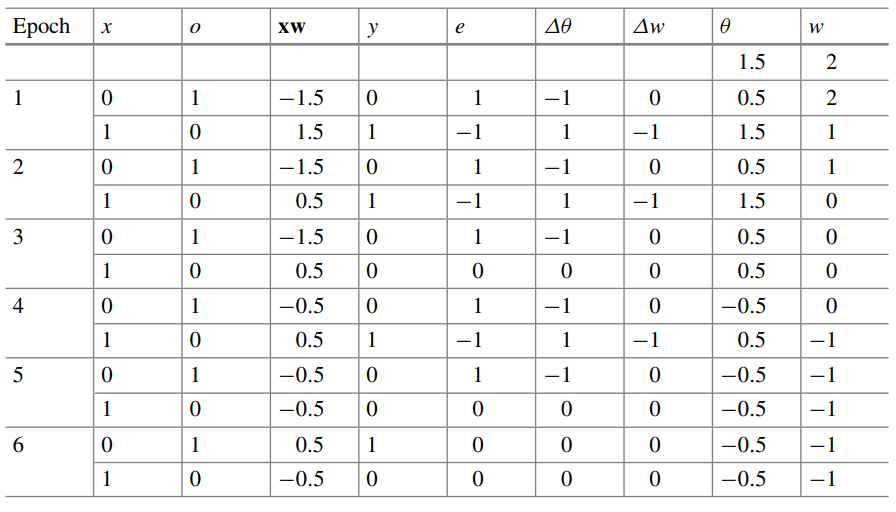
\includegraphics[scale=0.5]{images/online_training.png}
    \caption{Online training with $\theta = \frac{3}{2},w=2,\eta =1$}
\end{figure}

\begin{figure}[H]
    \centering
    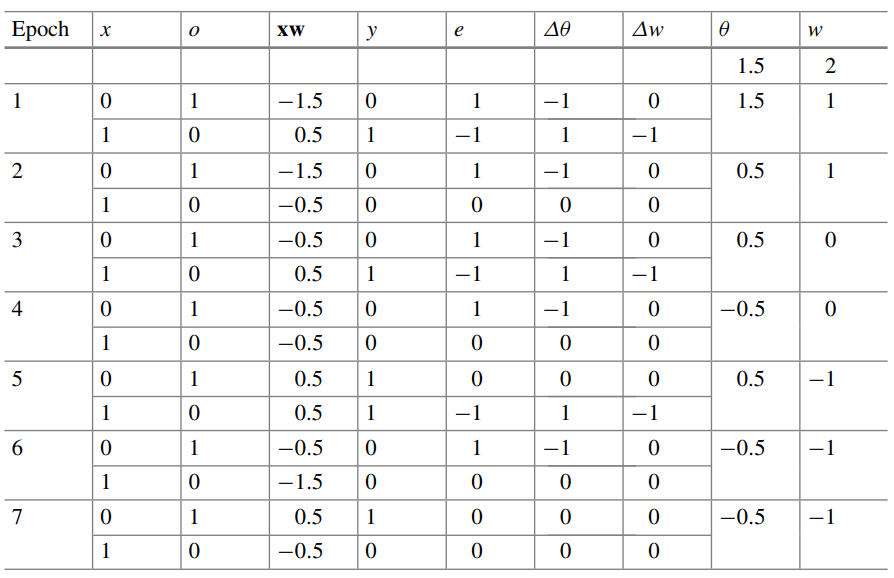
\includegraphics[scale=0.5]{images/batch_training.png}
    \caption{Batch training with $\theta = \frac{3}{2},w=2,\eta = 1$}
\end{figure}

Basically what happens in the online training, if i start in the first move i may go here,
and so on, i'll move one step at the time since the amount of change is control by the
learning rate.

in this case i move in one direction, since i apply together the two errors correction,
so i'm moving in combination of the two changes of the secondo batch, then again i'm applying
the two changes and i move. I do less move respect to the other since  i combine the two
correction for the expression that i shown.

I can try to do the same for the more complex case of the TLU, with two inputs. here i have
the conjunction with the truth table describing the implementation. What i'm doing basically
i have found the straight line that gives the satisfied and unsatisfied area for determining
the solution.

\subsubsection{Convergence theorem}
If we consider a set of training patterns: $L=\{(\vec{x},o_1),...,(\vec{x}_m,o_m)\}$,
each consisting of an input vector $\vec{x_i}\in\mathbb{R}$ and a desired
output $o_i\in\{0,1\}$.

Furthermore, let's consider $L_0=\{(\vec{x},o)\in L|o=0\}$ and
$L_1=\{(\vec{x},o)\in L | o=1\}$. If i can show that $L_0$ and $L_1$ are
\textbf{linearly separable}, then is possible to prove that we have a
$\vec{w}\in\mathbb{R}^n$ and $\theta\in\mathbb{R}$ such that:
$$\forall (\vec{x},0)\in L_0 :\vec{w}^T\vec{x} <\theta$$
$$\text{and}$$
$$\forall (\vec{x},1)\in L_0:\vec{w}^T\vec{x}\geq\theta$$

This means that is possible to divide the two sets, and then the online or batch
training procedure is able to terminate. So if the two sets are linearly separable they
will give us a final value in a \textbf{finite time}. The final error will e zero.

The problem is that if we are not able to perform the linear separation of $L_0$ and $L_1$,
the algorithm is \textbf{not able to terminate}. The algorithm will oscillate around and we
will not be able to find a solution with the zero error.

\begin{figure}[H]
    \centering
    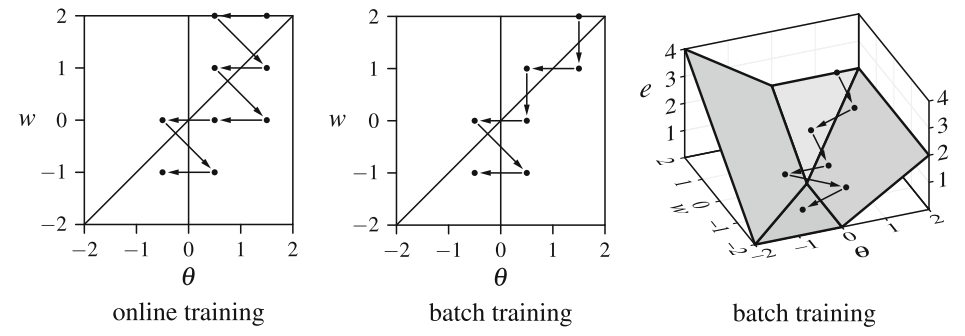
\includegraphics[scale=0.4]{images/batch_training_example_graph.png}
    \caption{Example of online and batch training (also with summed errors)}
\end{figure}

The correction of the parameters maybe slowed down due to the fact that we have $0$ and $1$
to the possible values for our outputs. This implies that if we have an output for our
threshold logic function equal to $1$, we can find an adjustment and apply it.
If we have an input which is $0$ whichever weight we have, we may not be able to compute
a correction that in the end will reduce the final error.

So when we apply an input which is one we can change the weight for finding a better value
for the configuration, if we apply the change on an input which is zero the possible changes
actually vanishes since we are multiplying by zero, we are not observing a variation.

To avoid to waste to much time on this issue, we can change the representation of the values,
for \textit{true} we are considering $1$ and for \textit{false} we are considering $-1$.

What we can point out, is that a \textit{single} TLU, is able to point out any linearly
separable function. We have just to apply the delta rule which is easy and fast and
guarantee to find a solution, if one exists.

The problem is given by a more complex structure, like a network of TLUs,
in this case we cannot apply directly the delta rule, because we have no clue
about which is the output. We need something more complex for managing that.

\subsection{Artificial neural network}
An ANN in general ha a very simple definition since it is a \textbf{directed}
graph $G=(U,C)$ composed by nodes and edges, in the graph we have processing
nodes that can elaborate the information incoming in, some arcs that
are bringing in the network some external information, and others that extract
the computation performed by our network (which is a structure that mimic our
brain).

The connections are the axon-synaptic connections which connect the nucleus of the
neurons. In a general neural network this is the very abstract definition, in practice
in order to use this kind of structure we will need to have more regular more focused
organization of neurons connections.

The set of vertices $U$ is partitioned into:
\begin{itemize}
    \item $U_{in}$ is the set of input neurons.
    \item $U_{out}$ is the set of output neurons, whi are the one delivering the
          result of the computation to the outside world.
    \item $U_{hidden}$ is the set of hidden neurons, they don't have any direct
          connection to the external world.
\end{itemize}

\subsubsection{General structure of the neuron}

\begin{figure}[H]
    \centering
    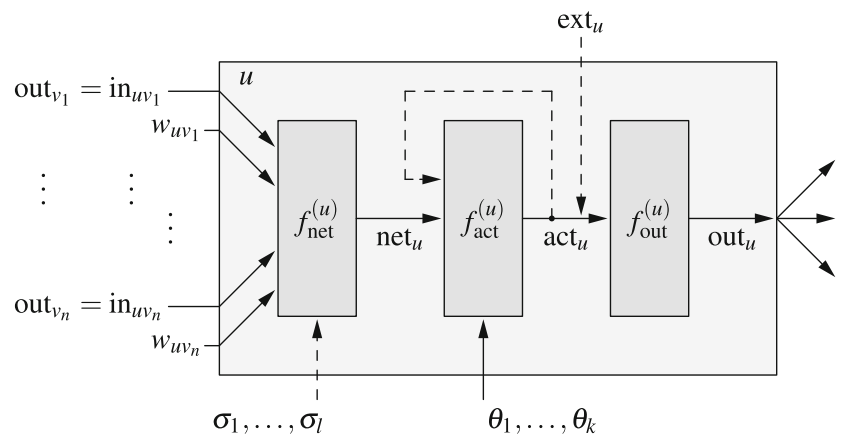
\includegraphics[scale=0.5]{images/general_structure_neuron.png}
    \caption{Internal representation of a neuron}
\end{figure}

We see that we have inputs that are coming in the network and usually this inputs are
manipulated in order to understand which is the global stimulus that the neuron
receive from the external world.

If an incoming signal from a previous neuron has relevance, we want to multiply the
amount o signal incoming in by an appropriate constant in order to have a stronger weight
for a subsequent processing in this neuron.

In this example we associate the weight $w_{uv_1}$, which is the weight for the neuron
$u$ respect to the incoming neuron $v_1$.

These inputs are processed by three stages in which we perform specific operations, we want
to see how much the neuron is actually solicited. For these reason we have three
stage functions:

\begin{itemize}
    \item The $f_{net}^{(u)}$, takes the input with the \textit{relative relevance} of the
          various inputs to generate the \textbf{global solicitation} for our neuron. This is a general
          definition, a specific definition changes in base of the network we are considering.

    \item The $f_{act}^{(u)}$, the activation functions analyze the network input from the
          previous function and generate the \textbf{excitation status} of our neuron. This will tell
          us if the neuron is sufficiently excited.

    \item The $f_{out}^{(u)}$, which takes the excitation status of the neuron and elaborate
          the final status of the neuron to deliver to the subsequent neurons.
\end{itemize}

In general we have also an external variable $ext_u$ which tell us how much the excitation
should be increased from a stimulus coming directly from the \textit{external world}
(not from previous neuron, from the external world).

These are the various inputs that any neuron can have, we may have both the input coming
from other neurons and the input coming from the external world, or we can have for a subset
of neurons only the stimulus coming from the external world and no other inputs.

We have input neurons coming which are weighted properly, these values are used
with the \textit{network input function} which is generating the global excitation status
coming from the other neurons, this one is will generate the \textit{activation status} of the neuron (how much it is
stimulated by the external neurons).

In the end we have the out function which evaluates the final status of the neuron, which
is delivered to the other connected neuron.

\subsubsection{Type of artificial neural network}
In the practice we won't use the general structure introduced before, we will have
different type of ANN:

\begin{itemize}
    \item \textbf{feed forward network} are ANN that doesn't contains any cycles, the
          acronym is FNN.
    \item \textbf{recurrent network} are ANN that contains cycles (backward connections),
          the acronym is RNN.
\end{itemize}

\noindent
The operation of a general ANN:
\begin{enumerate}
    \item \textbf{input phase}, where the external input are acquired by
          input neurons in the network.

    \item \textbf{work phase}, the external input are disconnect (by freezing
          the input neurons), we move the excitation generated by the input neurons
          to the connected neurons, we generate the stimuli for the connected neuron,
          we compute the output status of them and propagate the output to the
          neurons which are connected to this one.
\end{enumerate}

During the \textit{working phase} if the input of neurons are steady (input stimuli
are not changing), the computation of that neuron doesn't change (every stage
function generate the same values, FNN).

This is not the case when we have a RNN, since if one of the outputs connected to
a neuron is connected to an input will repeat the computation and this maybe change
the output status (due to \textit{recomputation}). I always say \textit{"may"}
since the actual change will depend specifically by the function that i'm using.
The \textbf{recomputation} of a neuron output occurs if any of its input changes,
we can't loop forever and not evolving. This means that the working phase continues
until the external outputs are steady, or a maximum number of
recomputation iterations is reached. The \textbf{temporal order} of computation
depends by the specific NN.
\newline
\newline
\noindent\textbf{Feed-forward neural network}
\begin{enumerate}
    \item Computation proceeds from input neurons progressively toward output neurons by following
          the topological order of the neuron in the network.
    \item The external inputs are frozen.
    \item Input neuron compute their outputs which are maintained steady and forwarded
          to the connected neurons.
    \item Neurons connected to preceding neurons with steady outputs generate their
          respective outputs and propagated forward to the subsequent neurons, until the
          external outputs are generated.
\end{enumerate}
\noindent\textbf{Recurrent neural network}
\begin{figure}[H]
    \centering
    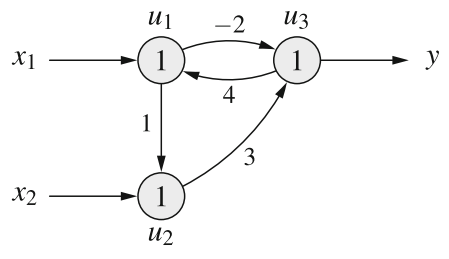
\includegraphics[scale=0.5]{images/RNN.png}
    \caption{A simple recurrent neural network}
\end{figure}
In the neurons there is the threshold which is considered for the operation,
and we have some interconnection weights which define the weights to be applied to the output
of a neuron when his output is delivered as input to a subsequent neuron.
\begin{figure}[H]
    \centering
    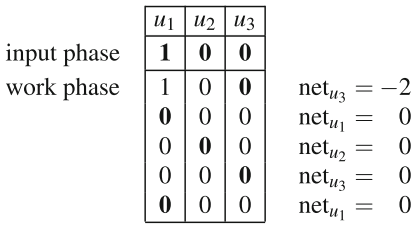
\includegraphics[scale=0.6]{images/RNN_simpl_ex1.png}
    \caption{Dataset for the previous RNN, for the $u_3,u_2,u_1$ order}
\end{figure}
In this case we choice to start from the input $1,0,0$ and with an updating order of
neurons that is $u_3,u_1,u_2,u_3,u_1,u_2,u_3,...$. Each bold number in working phase
entry of the table is an output of the \textit{ordered} neuron ($0$ if greater less than $\theta$
or viceversa $1$). In this case we can reach a steady state, and exit the RNN.
\begin{figure}[H]
    \centering
    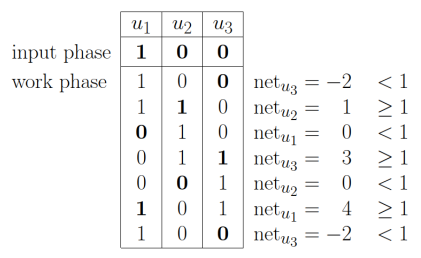
\includegraphics[scale=0.6]{images/RNN_simpl_ex2.png}
    \caption{Different dataset of the same RNN with $u_3,u_2,u_1$ order}
\end{figure}
Now let's consider a different ordering $u_3,u_2,u_1,u_3,u_2,u_1,u_3,...$, in this case
it is not possible to reach a steady state inside the RNN (\textbf{no stable state}, \textit{
    oscillation} of output).

\subsubsection{Configuration of a neural network}
The details of the configuration strictly depends from the
structure opf the network, in general we have two categories of
learning procedure (or training procedure):

\begin{itemize}
    \item \textbf{fixed learning task}.
    \item \textbf{free learning task}
\end{itemize}
\pagebreak
\noindent\textbf{Fixed learning task}
\newline
\noindent Considering a NN of $n$ input neurons $U_{in}=\{u_1,...,u_n\}$ and $m$ output neurons
$U_{out}=\{v_1,...,v_m\}$. A fixed learning task is a set of training patterns
$l=(\vec{i^{(l)}}, \vec{o^{(l)}})$, each consisting of:
\begin{itemize}
    \item an input vector $\vec{i^{(l)}} =(ext_{u_1}^{(l)},...,ext_{u_n}^{(l)})$
    \item an output vector $\vec{o^{(l)}} =(o_{v_1}^{(l)},...,o_{v_m}^{(l)})$.
\end{itemize}
\noindent At the end of the configuration the network is able to generate the desired output
that correspond to the output vector. Since the examples are composed by an input
vector and the expected output that we want to get, this is called \textbf{supervised
    learning}.

A fixed learning task is solved when for all training patterns $l\in L_{fixed}$ the
neural network computes, from the external inputs contained in the input vector
$\vec{i^{(l)}}$ of a training pattern $l$, the outputs contained in the
corresponding output vector $\vec{o^{(l)}}$.
\newline
\newline
\noindent\textbf{The error of a fixed learning task}
\newline
The error says how well a neural network solves a given fixed learning task. Essentially
it is the difference between desired and actual outputs.
$$e=\sum_{l\in L_{fixed}}e^{(l)}=\sum_{v\in U_{out}}e_v=\sum_{l\in L_{fixed}} \sum_{v\in U_{out}}e_v^{(l)}$$
$$e_v^{(l)}=\left(o_v^{(l)}-out_v^{(l)}\right)^2$$
In order to have a number which tell us the final quality what we need to do we have
to consider the module of the error, what we are doing is consider the difference between
the actual and the desired output. But in this simple difference could give us a final
number which is not reflecting the total accuracy of the NN due to the \text{sign}.

A solution to this is to use a squared value, in this way we can avoid the negative
sign.
\newline\newline\noindent\textbf{Free learning task}\newline
A free learning task is the complementary approach of the fixed learning task, in
which the desired behavior is not defined a priori by the pair of vectors for
the input and the output.

$$n\text{ input neurons }U_{in}=\{u_1,...,u_n\}$$
$$\text{one input vector }\vec{i^{(l)}} = \left( ext_{u_1}^{(l)},...,ext_{u_1}^{(l)}\right)$$

We only have a set of input vectors which are presented to the network and the
learning algorithm will lead to an output vector which is similar to the given input.

\noindent\newline\textbf{Preprocessing}\newline
In order to be sure that the learning is working properly, we have to be sure
that one of the input is dominating the operation of the network, as consequence
we have to do some preprocessing on the data in order to give the same relevance
to all neurons.

For each component of the input vector we need to compress the representation
in the same range, this is called \textbf{normalization} (according to the
average of the input value for each component, we need to be sure that
the variance $\sigma_k$ is normalized as well).
$$\mu_k =\frac{1}{|L|}\sum_{l\in L}ext_{u_k}^{(l)}$$
$$\sigma_k =\sqrt{\frac{1}{|L|-1}\sum_{i\in L}\left(ext_{u_k}^{(l)}-\mu_k\right)^2}$$

This is the standard normalization of the deviation $\sigma_k$, we have also another
possibility which is called \textbf{unbiased standard deviation} (often preferred
by statistician since is not polarized on the two direction).

If we apply the normalization this is the external stimuli that we will have after
the normalization, basically all the stimuli are recomputed with respect to the
average value and they are normalized in dimension dividing them by the standard
deviation.
$$\sigma_{u_k}^{(l)(new)}=\frac{ext_{u_k}^{(l)(old)}-\mu_k}{\sigma_k}$$

There is a problem that we have to seriously consider when we are looking
to our examples, we need to have \textit{sufficiently descriptive examples},
which have to be well distributed over the domain that i'm considering (not
focussing only on a portion of the domain).

So far we have been dealing with integer and real numbers, we want to use
symbols for represent a group of examples that are similar together in a concise way.

For doing that we need to associate a group of identifiers to a group of examples. For
being able to represent this symbols we consider the \textbf{1-in-N encoding}, if
we need to represent $n$ symbols we have a string of $0$ and $1$ and only one bit the one
that corresponds to the symbol we want to represent will be $1$ (the others will be $0$).

\end{document}